\section{Theory}

	By using the excitation of neon atoms in a cathode tube and recording the excitation energy necessary for the transition between the states, the Frank Hertz experiment confirms the quantization of energy states. Thus, using Plank's (Blackbody radiation) and Einstein's new quantum theory, Frank Hertz was used as a verification for Bohr's atomic model for the hydrogen spectrum (Photoelectric effect).

	The thermionic emission process, which is heated by a filament in the tube's cathode to emit electrons, is used to excite the neon atoms through inelastic collisions. A knob is used to regulate the heating voltage. Electrons in Ne atoms are excited and then de-excited to produce a direct-observable glow in the gas after absorbing energy from collisions. The ten 3p-states, which are between 18.4 eV and 19.0 eV above the ground state, are where the most likely excitation through inelastic electron collision occurs, as shown in the following figure. The probability of excitation is lower for the four lower 3s-states between 16.6 eV and 16.9 eV. Only through the 3s-states are the 3p states able to be de-excited to the ground. An photon is released as a result of the 3p-3s transition. This process emits light that is visible to the human eye and falls in the region between red and green.

	Between the cathode K and the anode A is the accelerating voltage UA. Through an inelastic collision, the emitted electrons excite the neon atoms, and depending on their kinetic energy, they then fall on electrode E and contribute to the collector current. As the accelerating potential rises, the collector current also rises while the other voltages (UF, UKG, and UAE) remain constant. When the electrons are moving closely in front of Anode A and have just enough kinetic energy to transfer the energy needed to excite the neon atoms through collisions, the collector current is at its highest. Because the electrons after a collision can no longer overcome the braking voltage UAE present between anode A and collector electrode E, the collector current drops off dramatically. The luminous zones that are observed at the distances where the atoms are excited are the minima. The electrons reach the energy level necessary for exciting the neon atoms at ever-greater distances from anode A as the acceleration voltage UA rises.
	
	\begin{figure}[H]
		\centering
		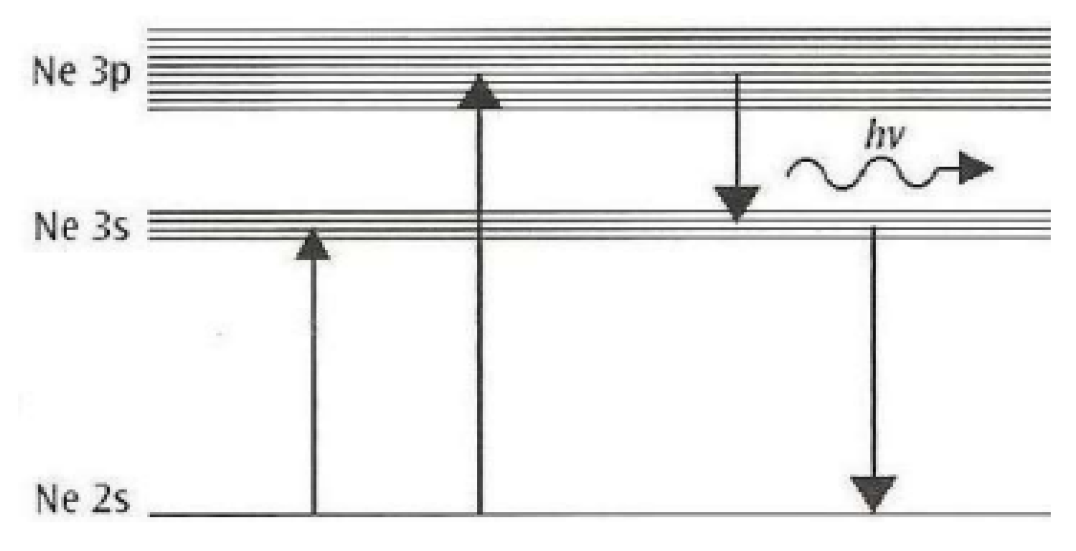
\includegraphics[width=0.3\textwidth]{1.png}
		\caption{\textbf{Energy level diagram for Neon}}
		\label{fig:1}
	\end{figure}

	As a result, the emission line is already obtained. After colliding, they are once again accelerated, and when the acceleration voltage is enough, they once more absorb enough energy from the electrical field to excite a neon atom, resulting in the formation of more than one maximum. As shown in the figure below, at higher acceleration voltages, we can see distinct red/orange luminance layers between grid G and anode A. The distance between the equidistant maxima of the electron current in a variable opposing electric field is used to calculate the excitation energy of neon.
	
	\begin{figure}[H]
		\centering
		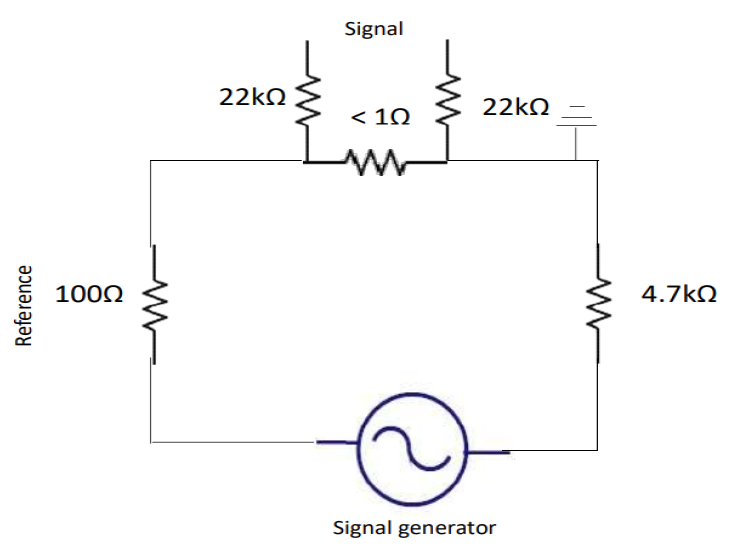
\includegraphics[width=0.3\textwidth]{2.png}
		\caption{\textbf{Visible luminescence layers between grids}}
		\label{fig:2}
	\end{figure}



\section{Experimental Setup}
	As shown in figure below, the Franck-Hertz tube is a tetrode with an indirectly heated barium oxide cathode K, a meshtype control grid G, a mesh-type anode A, and a collector electrode E. The electrodes are in a planeparallel configuration and the tube is fileld with neon gas at a pressure appropriate for the characteristic curve (several hundred Pascal). The distance between the control grid and the anode grid is about 5 mm, and the distances between the cathode and the control grid and between the anode and the collector electrode are both about 2 mm.
	
	\begin{figure}[H]
		\centering
		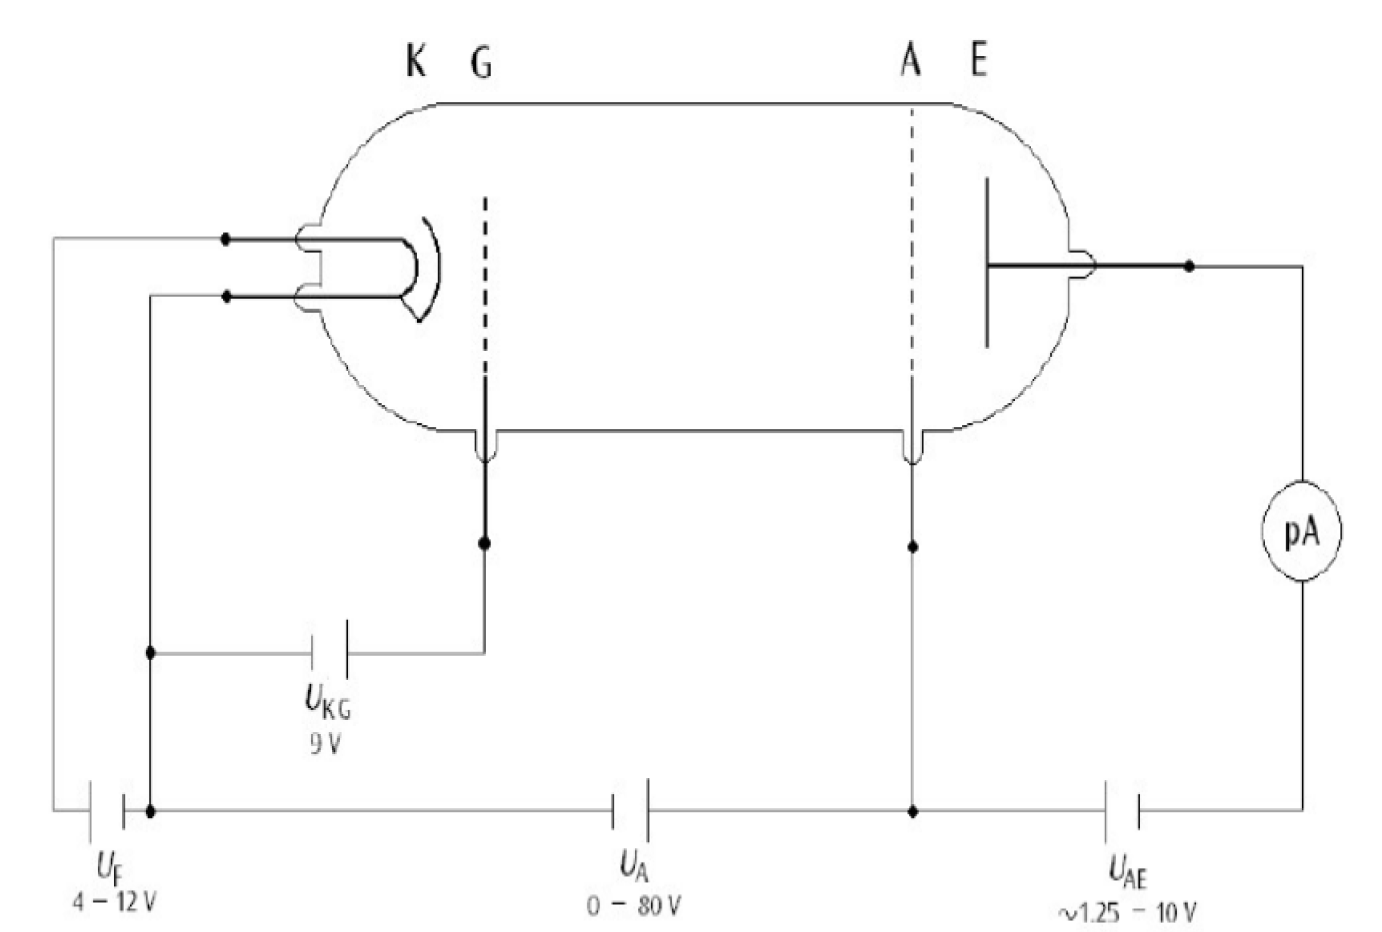
\includegraphics[width=0.35\textwidth]{3.png}
		\caption{\textbf{Frank-Hertz tube setup and circuit diagram}}
		\label{fig:3}
	\end{figure}

	The connecting sockets for the heater (Filament voltage: 4 - 12 V), control grid (Control voltage: 9 V) and anode grid voltages are on the base of the instrument. The collector current is taken off through the BNC socket at the top end of the screening cylinder. An internal $10k\ohm$ limiting resistor is permanently built in between the connector sockets for the accelerator (control grid) voltage and the anode voltage. This protects the tube in case there is a spark discharge caused by applying too high a voltage. The voltage loss in this resistor when making measurements is negligible, as the anode current in the tube is smaller than 5 pA. (Thus the voltage loss in the protecting resistor is 0.05 V.)
